\documentclass[journal,12pt,twocolumn]{IEEEtran}

\usepackage{setspace}
\usepackage{gensymb}
\singlespacing
\usepackage[cmex10]{amsmath}

\usepackage{amsthm}

\usepackage{mathrsfs}
\usepackage{txfonts}
\usepackage{amsmath}
\usepackage{stfloats}
\usepackage{float} 
\usepackage{bm}
\usepackage{tikz}
\usepackage{pgfplots}
\usepackage{cite}
\usepackage{cases}
\usepackage{subfig}

\usepackage{longtable}
\usepackage{multirow}

\usepackage{enumitem}
\usepackage{mathtools}
\usepackage{steinmetz}
\usepackage{tikz}
\usepackage{circuitikz}
\usepackage{verbatim}
\usepackage{tfrupee}
\usepackage[breaklinks=true]{hyperref}
\usepackage{graphicx}
\usepackage{tkz-euclide}

\usetikzlibrary{calc,math}
\usepackage{listings}
    \usepackage{color}                                            %%
    \usepackage{array}                                            %%
    \usepackage{longtable}                                        %%
    \usepackage{calc}                                             %%
    \usepackage{multirow}                                         %%
    \usepackage{hhline}                                           %%
    \usepackage{ifthen}                                           %%
    \usepackage{lscape}     
\usepackage{multicol}
\usepackage{chngcntr}
\usepackage{hyperref}
\hypersetup{
    colorlinks=true,
    linkcolor=blue,
    filecolor=blue,      
    urlcolor=blue,
}
\DeclareMathOperator*{\Res}{Res}

\renewcommand\thesection{\arabic{section}}
\renewcommand\thesubsection{\thesection.\arabic{subsection}}
\renewcommand\thesubsubsection{\thesubsection.\arabic{subsubsection}}

\renewcommand\thesectiondis{\arabic{section}}
\renewcommand\thesubsectiondis{\thesectiondis.\arabic{subsection}}
\renewcommand\thesubsubsectiondis{\thesubsectiondis.\arabic{subsubsection}}


\hyphenation{op-tical net-works semi-conduc-tor}
\def\inputGnumericTable{}                                 %%

\lstset{
%language=C,
frame=single, 
breaklines=true,
columns=fullflexible
}

\makeatletter
\setlength{\@fptop}{0pt}
\makeatother

\begin{document}


\newtheorem{theorem}{Theorem}[section]
\newtheorem{problem}{Problem}
\newtheorem{proposition}{Proposition}[section]
\newtheorem{lemma}{Lemma}[section]
\newtheorem{corollary}[theorem]{Corollary}
\newtheorem{example}{Example}[section]
\newtheorem{definition}[problem]{Definition}

\newcommand{\BEQA}{\begin{eqnarray}}
\newcommand{\EEQA}{\end{eqnarray}}
\newcommand{\define}{\stackrel{\triangle}{=}}
\bibliographystyle{IEEEtran}
\raggedbottom
\setlength{\parindent}{0pt}
\providecommand{\mbf}{\mathbf}
\providecommand{\pr}[1]{\ensuremath{\Pr\left(#1\right)}}
\providecommand{\qfunc}[1]{\ensuremath{Q\left(#1\right)}}
\providecommand{\sbrak}[1]{\ensuremath{{}\left[#1\right]}}
\providecommand{\lsbrak}[1]{\ensuremath{{}\left[#1\right.}}
\providecommand{\rsbrak}[1]{\ensuremath{{}\left.#1\right]}}
\providecommand{\brak}[1]{\ensuremath{\left(#1\right)}}
\providecommand{\lbrak}[1]{\ensuremath{\left(#1\right.}}
\providecommand{\rbrak}[1]{\ensuremath{\left.#1\right)}}
\providecommand{\cbrak}[1]{\ensuremath{\left\{#1\right\}}}
\providecommand{\lcbrak}[1]{\ensuremath{\left\{#1\right.}}
\providecommand{\rcbrak}[1]{\ensuremath{\left.#1\right\}}}
\theoremstyle{remark}
\newtheorem{rem}{Remark}
\newcommand{\sgn}{\mathop{\mathrm{sgn}}}
\providecommand{\abs}[1]{$\left\vert#1\right\vert$}
\providecommand{\res}[1]{\Res\displaylimits_{#1}} 
\providecommand{\norm}[1]{$\left\lVert#1\right\rVert$}
%\providecommand{\norm}[1]{\lVert#1\rVert}
\providecommand{\mtx}[1]{\mathbf{#1}}
\providecommand{\mean}[1]{$E\left[ #1 \right]$}
\providecommand{\fourier}{\overset{\mathcal{F}}{ \rightleftharpoons}}
%\providecommand{\hilbert}{\overset{\mathcal{H}}{ \rightleftharpoons}}
\providecommand{\system}{\overset{\mathcal{H}}{ \longleftrightarrow}}
	%\newcommand{\solution}[2]{\textbf{Solution:}{#1}}
\newcommand{\solution}{\noindent \textbf{Solution: }}
\newcommand{\cosec}{\,\text{cosec}\,}
\providecommand{\dec}[2]{\ensuremath{\overset{#1}{\underset{#2}{\gtrless}}}}
\newcommand{\myvec}[1]{\ensuremath{\begin{pmatrix}#1\end{pmatrix}}}
\newcommand{\mydet}[1]{\ensuremath{\begin{vmatrix}#1\end{vmatrix}}}
\newcommand*{\permcomb}[4][0mu]{{{}^{#3}\mkern#1#2_{#4}}}
\newcommand*{\perm}[1][-3mu]{\permcomb[#1]{P}}
\newcommand*{\comb}[1][-1mu]{\permcomb[#1]{C}}
\numberwithin{equation}{subsection}
\makeatletter
\@addtoreset{figure}{problem}
\makeatother
\let\StandardTheFigure\thefigure
\let\vec\mathbf
\renewcommand{\thefigure}{\theproblem}
\def\putbox#1#2#3{\makebox[0in][l]{\makebox[#1][l]{}\raisebox{\baselineskip}[0in][0in]{\raisebox{#2}[0in][0in]{#3}}}}
     \def\rightbox#1{\makebox[0in][r]{#1}}
     \def\centbox#1{\makebox[0in]{#1}}
     \def\topbox#1{\raisebox{-\baselineskip}[0in][0in]{#1}}
     \def\midbox#1{\raisebox{-0.5\baselineskip}[0in][0in]{#1}}
\vspace{3cm}
\title{Gate Assignment 1}
\author{Sachin Karumanchi - AI20BTECH11013}
\maketitle
\newpage
\bigskip
\renewcommand{\thefigure}{\theenumi}
\renewcommand{\thetable}{\theenumi}
Download all python codes from
\begin{lstlisting}
https://github.com/sachinkarumanchi/EE3900/tree/Gate_assignment1.ipynb
\end{lstlisting}
and latex codes from
\begin{lstlisting}
https://github.com/sachinkarumanchi/EE3900/tree/Gate_assignment1.tex
\end{lstlisting}
\section*{Problem}
Let $h[n]$ be a length-7 discrete-time finite impulse response filter, given by $h[0]=4$, $h[1]=3$, $h[2]$=2, $h[3]=1$, $h[-1]=-3$, $h[-2]=-2$, $h[-3]=-1$, and $h[n]$ is zero for $|n|\geq 4$. A length-3 finite impulse response approximation $g[n]$ of $h[n]$ has to be obtained such that
$$E(h,g)=\int_{-\pi}^{\pi}\left|H(e^{j\omega})-G(e^{j\omega})\right|^2d\omega$$
is minimized, where $H(e^{j\omega})$ and $G(e^{j\omega})$ are the discrete-time Fourier transforms of $h[n]$ and $g[n]$ respectively, For the filter minimizes $E(h,g)$, the value of 10$g[-1]$+$g[1]$, rounded off to 2 decimal places, is
\section*{Solution}
Consider $y[n]$ such that 
\begin{align}
    y[n]&=h[n]-g[n]
\end{align}
Let $Y(e^{j\omega})$ be the Discrete-time Fourier transform of $y[n]$.\\
From Parseval's theorem,
\begin{align}
    \sum_{n=-\infty}^{\infty}|x[n]|^2&=\frac{1}{2\pi}\int_{-\pi}^{\pi}\left|X(e^{j\omega})\right|^2d\omega \label{eq1}
\end{align}
from \eqref{eq1} we can say that
\begin{align}
    \int_{-\pi}^{\pi}\left|Y(e^{j\omega})\right|^2d\omega&=2\pi\sum_{n=-\infty}^{\infty}|y[n]|^2\\
    \int_{-\pi}^{\pi}\left|H(e^{j\omega})-G(e^{j\omega})\right|^2d\omega&=2\pi\sum_{n=-\infty}^{\infty}|y[n]|^2\\
    E(h,g)&=2\pi\sum_{n=-\infty}^{\infty}|y[n]|^2
\end{align}
Given that $h[n]$ is of length 7 and $g[n]$ is of length 3, also that $E(h,g)$ to be minimum.\\
Therefore, $E(h,g)$ transforms into
\begin{align}
    E(h,g)&=2\pi\sum_{n=-3}^{3}|h[n]-g[n]|^2
\end{align}
\begin{multline}
    E(h,g)=2\pi(|4-g[0]|^2+|3-g[1]|^2+\\|-3-g[-1]|^2+10)
\end{multline}
The values of $g[0]=4$, $g[1]=3$, $g[-1]=-3$ for $E(h,g)$ to be minimum.\\
Now, finding the value of 10$g[-1]$+$g[1]$
\begin{align}
    10g[-1]+g[1]&=10\times (-3)+3\\
    &=-27
\end{align}
The value of 10$g[-1]$+$g[1]$ is -27.00
\begin{figure}[h]
    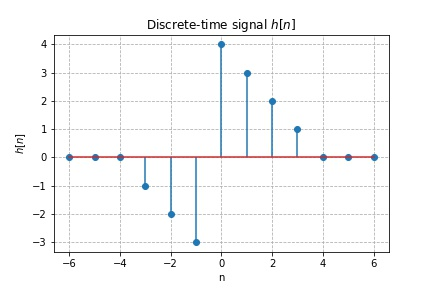
\includegraphics[width=10cm]{h[n] signal.jpg}
\end{figure}
\begin{figure}[h]
    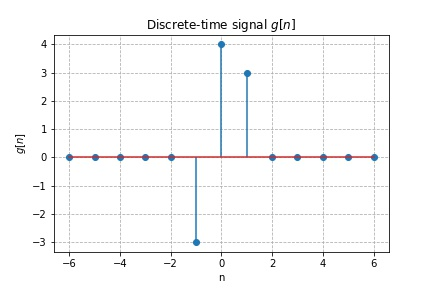
\includegraphics[width=11cm]{g[n] signal.jpg}
\end{figure}
\end{document}